
% Preamble
\documentclass[11pt]{article}

\newcommand*{\srcDirectory}{src}
\newcommand*{\importDirectory}{imports}
\newcommand*{\settingsDirectory}{settings}
\newcommand*{\tikzDirectory}{tikz}
\newcommand*{\importDirectDirectory}{\srcDirectory/\importDirectory}
\newcommand*{\settingsDirectDirectory}{\srcDirectory/\settingsDirectory}
\newcommand*{\tikzDirectDirectory}{\srcDirectory/\tikzDirectory}


\usepackage{enumitem}
\usepackage{hyperref}
\usepackage[T1]{fontenc}
\usepackage[polish]{babel}
\usepackage{lmodern}
\usepackage{geometry}

\geometry{
    paperheight=185.625mm,
    paperwidth=297mm,
    left=20mm,
    right=20mm,
    top=20mm,
    bottom=20mm
}
\usepackage{fancyhdr}
\pagestyle{fancy}
\fancyhf{}
\fancyfoot[R]{\thepage}
\renewcommand{\headrulewidth}{0pt}
\renewcommand{\footrulewidth}{0pt}

%https://www.reddit.com/r/GradSchool/comments/cmfxjm/i_just_discovered_how_to_make_darkmode_pdfs_in/

\usepackage{xcolor}
\pagecolor[rgb]{0,0,0} %black
\color[rgb]{0.5,0.5,0.5} %grey
\usepackage{amsmath}
\usepackage{amssymb}
\usepackage{tikz}
\usetikzlibrary{shapes,fit,matrix,snakes}
\usepackage{standalone}
\tikzset{
 point/.style={circle=1mm,fill=red!60!black,scale=0.5}
}
\pgfdeclarelayer{bg}
\pgfsetlayers{bg,main} 

%https://tex.stackexchange.com/questions/58903/how-to-draw-star-in-tikz-background
\newcommand{\tstar}[6]{% inner radius, outer radius, tips, rot angle, options, name
    \pgfmathsetmacro{\starangle}{360/#3}
    \draw[#5] (#4:#1) coordinate (#6-0-0)
    \foreach \x in {1,...,#3} { 
        -- (#4+\x*\starangle-\starangle/2:#2) coordinate (#6-\x-0) 
        -- (#4+\x*\starangle:#1)              coordinate (#6-\x-1)
    }
    -- cycle;
}

%https://tex.stackexchange.com/questions/58903/how-to-draw-star-in-tikz-background
\newcommand{\ngram}[5]{% outer radius, tips, rot angle, options
    \pgfmathsetmacro{\starangle}{360/#2}
    \pgfmathsetmacro{\innerradius}{#1*sin(90-\starangle)/sin(90+\starangle/2)}
    \tstar{\innerradius}{#1}{#2}{#3}{#4}{#5}
}



\begin{document}

\thispagestyle{empty}
    \null
    \vspace{5cm}
    \begin{center}
        \begin{Huge}
            \fontsize{50pt}{50pt}\selectfont{Otoczki wypukłe wielokąta prostego}
        \end{Huge}
    \end{center}
    \vspace{5cm}
    
   \begin{flushright}
   
   \Huge{Marcin Belicki} 
   \end{flushright}
        
    
    \newpage
    \begin{center}
        \begin{Huge}
            \fontsize{46pt}{46pt}\selectfont{Definicja}
        \end{Huge}   
    \end{center}
    \begin{LARGE}
        \textbf{Otoczka wypukła} - dla zbioru punktów $Z\subset\mathbb{R}^2$ jest to wielokąt wypukły $H(Z)$, taki że zawiera w swoim wnętrzu lub na krawędziach wszystkie punkty $p\in Z$, a przy tym mając pole najmniejsze z możliwych.
        \begin{center}
            \includestandalone[height = 10 cm]{\tikzDirectDirectory/1}
        \end{center}    
    \end{LARGE}   
    
    \newpage
    \begin{center}
    \begin{Huge}
        \fontsize{46pt}{46pt}\selectfont{Zastosowania}
    \end{Huge}   
\end{center}
\begin{LARGE}
    Właściwości otoczki wypukłej można wykorzystać w grafice komputerowej. 
    Przykładem tego może być wykrywanie przez silnik graficzny kolizji między obiektami.
    Jeśli wiemy, że obiekt czeka kolizja z płaską powierzchnią możemy przyjąć,
    że kolizja nastąpi wtedy i tylko wtedy gdy nastąpi kolizja otoczki wypukłej tego obiektu z powierzchnią.
\end{LARGE}
\begin{center}
    \includestandalone{\tikzDirectDirectory/2_0}
\end{center} 

    \newpage
    \begin{center}
    \begin{Huge}
        \fontsize{46pt}{46pt}\selectfont{Zastosowania}
    \end{Huge}   
\end{center}
\begin{LARGE}
    Właściwości otoczki wypukłej można wykorzystać w grafice komputerowej. 
    Przykładem tego może być wykrywanie przez silnik graficzny kolizji między obiektami.
    Jeśli wiemy, że obiekt czeka kolizja z płaską powierzchnią możemy przyjąć,
    że kolizja nastąpi wtedy i tylko wtedy gdy nastąpi kolizja otoczki wypukłej tego obiektu z powierzchnią.
\end{LARGE}
\begin{center}
    \includestandalone{\tikzDirectDirectory/2_1}
\end{center}

    \newpage
    \begin{center}
    \begin{Huge}
        \fontsize{46pt}{46pt}\selectfont{Zastosowania}
    \end{Huge}   
\end{center}
\begin{LARGE}
    Właściwości otoczki wypukłej można wykorzystać w grafice komputerowej. 
    Przykładem tego może być wykrywanie przez silnik graficzny kolizji między obiektami.
    Jeśli wiemy, że obiekt czeka kolizja z płaską powierzchnią możemy przyjąć,
    że kolizja nastąpi wtedy i tylko wtedy gdy nastąpi kolizja otoczki wypukłej tego obiektu z powierzchnią.
\end{LARGE}
\begin{center}
    \includestandalone{\tikzDirectDirectory/2_2}
\end{center}

    \newpage
    \begin{center}
    \begin{Huge}
        \fontsize{46pt}{46pt}\selectfont{Zastosowania}
    \end{Huge}   
\end{center}
\begin{LARGE}
    Właściwości otoczki wypukłej można wykorzystać w grafice komputerowej. 
    Przykładem tego może być wykrywanie przez silnik graficzny kolizji między obiektami.
    Jeśli wiemy, że obiekt czeka kolizja z płaską powierzchnią możemy przyjąć,
    że kolizja nastąpi wtedy i tylko wtedy gdy nastąpi kolizja otoczki wypukłej tego obiektu z powierzchnią.
\end{LARGE}
\vspace*{\fill}
\begin{center}
    \includestandalone{\tikzDirectDirectory/2_3}
\end{center}

    \newpage
    \begin{center}
    \begin{Huge}
        \fontsize{46pt}{46pt}\selectfont{Zastosowania}
    \end{Huge}   
\end{center}
\begin{LARGE}
    Dzięki reprezentacji obiektu przez jego otoczkę wypukłą uzyskujemy mniej skomplikowany wielokąt,
    przez co łatwiej jest przeprowadzić nam obliczenia potrzebne do wykrycia kolizji.
\end{LARGE}
\vspace*{\fill}
\begin{center}
    \includestandalone{\tikzDirectDirectory/2_3}
\end{center}

    \newpage
    \begin{center}
    \begin{Huge}
        \fontsize{46pt}{46pt}\selectfont{Zastosowania}
    \end{Huge}   
    \end{center}
    \begin{LARGE}        
        Otoczka wypukła może okazać się również bardzo przydatna w kartografii. Używa się jej na przykład do generalizacji obszarów. Choć sama otoczka obszaru Polski nie jest zbyt dobrą jej reprezentacją to możemy wyznaczyć również otoczki wypukłe obszarów utworzonych przez krawędzie otoczki wypykłej oraz punkty zawarte ,,pod'' odpowiednimi krawędziami. W ten sposób możemy rekurencyjnie uzyskać coraz dokładniejszy obszar. Dzięki czemu jesteśmy w stanie  kontrolować dokładność w zależności od naszych potrzeb.
        \vspace*{\fill}
        \begin{center}
            \includestandalone{\tikzDirectDirectory/3}
            \hspace{1cm}
            \includestandalone{\tikzDirectDirectory/convex}
            \hspace{1cm}
            \includestandalone{\tikzDirectDirectory/convex2}
        \end{center} 
    \end{LARGE}  
    
    \newpage
    \begin{center}
    \begin{Huge}
        \fontsize{46pt}{46pt}\selectfont{Zastosowania}
    \end{Huge}   
    \end{center}
    \begin{LARGE} 
        Kolejnym przykładem obszaru zastosowania otoczki wypukłej może być przetwarzanie sygnałów. Często zdarza się w przypadku badania sygnałów okresowych, że przebieg samego sygnału nie niesie ze sobą zbyt wielu bezpośrednich informacji. Dlatego też w celu analizy właściwości   amplitudy sygnału potrzebna jest jego obwiednia. Dzięki wykorzystaniu otoczki wypukłej jesteśmy w stanie rekurencyjnie wyznaczyć punkty należące do obwiedni.        
        \begin{center}
            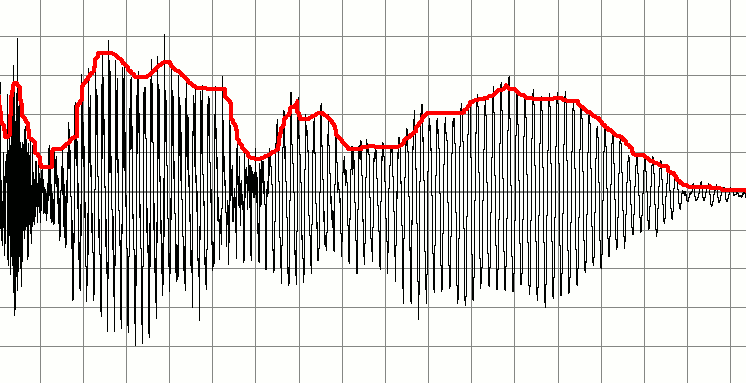
\includegraphics[decodearray={0.6 0 0.6 0 0.6 0},height=8cm]{\srcDirectory/envelope}
        \end{center} 
    \end{LARGE} 

    \newpage
    \begin{center}
    \begin{Huge}
        \fontsize{46pt}{46pt}\selectfont{Algorytm wyznaczania otoczki wypukłej wielokąta prostego}
    \end{Huge}   
    \end{center}
    \begin{Large} 
        \begin{minipage}{0.4\textwidth}
            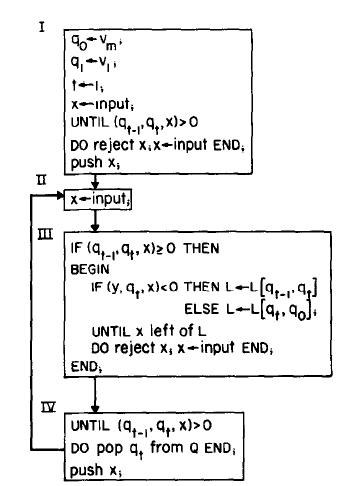
\includegraphics[decodearray={0.6 0 0.6 0 0.6 0},height=11cm]{1}
        \end{minipage}
        \begin{minipage}{0.6\textwidth}
            W swoim artykule Ronald L. Graham oraz F. Frances Yao przedstawili algorytm wyznaczający otoczkę wypukłą wielokąta prostego w czasie liniowym. Jest to istotne, zwłaszcza ze względu na fakt, iż wiadome jest, że wyznaczenie otoczki wypukłej zbioru punktóww ma złożoność czasową $O\left(n \log n\right)$. W celu zastosowania algorytmu LeftHull, wielokąt należy wstępnie przetworzyć - to jest podzielić na dwa wielokąty prostą łączącą dwa skrajne punkty (które na pewno wyznaczać). Następnie po przeprowadzeniu algorytmu dla każdej z tych części rozwiązania należy połączyć.\\
            Założenia:\\
            Punkty są uporządkowane w kolejności zgodnie ze wskazówkami zegara.\\
            $$\left(a,b,c\right) = \left\{
                \begin{array}{cl}
                    1 & \text{dla punktu $c$ leżącego na prawo od prostej $ab$}\\    
                    0 & \text{dla punktu $c$ leżącego na prostej $ab$}\\      
                    -1 & \text{dla punktu $c$ leżącego na lewo od prostej $ab$}   
                \end{array}
                
                
                \right.$$
        \end{minipage}
    \end{Large} 

    \newpage
    \begin{center}
    \begin{Huge}
        \fontsize{46pt}{46pt}\selectfont{Źródła}
    \end{Huge}   
    \end{center}
    \begin{large} 
        \begin{enumerate}[label={[\arabic*]}]
        
            \item Ronald L. Graham, Frances Yao, Finding the Convex Hull of a Simple Polygon (1981)
            \item \url{https://pl.wikipedia.org/wiki/Obwiednia_sygna%C5%82u#/media/Plik:C_Envelope_follower.png}
               [dostęp: 27.11.2021 10:29] 
            \item John Hershberg, Jack Snoeyink, Cartographic line simplification and polygon CSG formula in $O\left(n\log^* n\right)$ time (1997 - 1998)
            \item \url{https://gis-support.pl/wp-content/uploads/CNTR_RG_01M_2016_4326.shp_.zip}
               [dostęp: 27.11.2021 10:47] 
        \end{enumerate}
    \end{large} 


\end{document}